% =====================================================================
%  Project B report - AIAA conference paper layout
%  Author: Maxat Bekmurzayev
%
%  Compile:  pdflatex report.tex   (run twice)
%  Figures are read from ../results
% =====================================================================
\documentclass[letterpaper,10pt]{article}

\usepackage[margin=1in]{geometry}
\usepackage[T1]{fontenc}
\usepackage{mathptmx}
\usepackage{amsmath}
\usepackage{bm}
\usepackage{graphicx}
\usepackage{booktabs}
\usepackage{array}
\usepackage{float}
\usepackage[labelsep=space,labelfont=bf,font=small]{caption}
\usepackage{subcaption}
\usepackage{titlesec}
\usepackage{enumitem}
\usepackage{xcolor}
\usepackage{siunitx}
\usepackage[hidelinks]{hyperref}

\graphicspath{{../results/}{results/}}
\sisetup{per-mode=symbol}

\renewcommand{\thesection}{\Roman{section}}
\renewcommand{\thesubsection}{\Alph{subsection}}
\renewcommand{\thesubsubsection}{\arabic{subsubsection}}
\titleformat{\section}[block]{\centering\normalsize\bfseries}{\thesection.}{0.5em}{}
\titleformat{\subsection}[block]{\normalsize\bfseries}{\thesubsection.}{0.5em}{}
\titleformat{\subsubsection}[block]{\normalsize\itshape}{\thesubsubsection.}{0.5em}{}
\titlespacing*{\section}{0pt}{12pt}{6pt}
\titlespacing*{\subsection}{0pt}{9pt}{4pt}

\captionsetup[figure]{name=Fig.}
\setlength{\parskip}{0pt}
\setlength{\parindent}{1.5em}

\newcommand{\figref}[1]{Fig.~\ref{#1}}
\newcommand{\vv}[1]{\bm{#1}}
\newcommand{\Tp}{^{\mathsf{T}}}

% =====================================================================
\begin{document}

\begin{center}
{\LARGE\bfseries Rendezvous and Docking Guidance for a Chaser Spacecraft\\[2pt]
in Low Earth Orbit\par}
\vspace{12pt}
{\large Maxat Bekmurzayev\footnote{Undergraduate student, L.~N.~Gumilyov Eurasian National University, Astana, Kazakhstan.}\par}
\end{center}

\vspace{6pt}
\begin{quote}
\bfseries
This report describes guidance for a \SI{1000}{kg} chaser spacecraft that
has to meet a target in a \SI{400}{km} circular orbit and dock with it.
For long distances I used the linear Hill--Clohessy--Wiltshire (HCW) equations
and impulsive maneuvers: phasing, Hohmann transfer and radial hop. For the
last \SI{100}{m} I used a glide-slope reference and a PD controller with
feedforward of the orbital terms. Three scenarios were simulated in MATLAB. A
rendezvous from \SI{50}{km} behind on the same orbit costs
\SI{2.770}{m/s} in \SI{5.73}{h}. A rendezvous from
\SI{100}{km} behind and \SI{2.5}{km} below the target costs
\SI{2.789}{m/s} in \SI{7.97}{h}. The terminal approach reaches the port
after \SI{9.2}{min} at \SI{0.100}{m/s}. The full mission needs
\SI{3.114}{m/s} and \SI{1.442}{kg} of propellant. I also found that at large
distances the HCW equations must be used in curvilinear coordinates: with
Cartesian coordinates the error after three orbits from \SI{50}{km} was
\SI{21}{km}, and with curvilinear coordinates \SI{25.0}{m}.
\end{quote}

% ---------------------------------------------------------------------
\section*{Nomenclature}
\begin{tabular}{@{}l@{\hspace{1.2em}=\hspace{1.2em}}l@{}}
$x, y, z$ & radial, along-track and cross-track position of the chaser, m \\
$a$ & target orbit radius, m \\
$n$ & mean motion, $\sqrt{\mu/a^3}$, rad/s \\
$T$ & orbital period, s \\
$\Phi$ & HCW state transition matrix \\
$\Delta v$, $\Delta V$ & single impulse, total delta-V, m/s \\
$\delta a$ & difference in orbit radius, m \\
$s$ & range along the approach axis, m \\
$K_p$, $K_d$ & proportional and derivative gains \\
$\omega_n$, $\zeta$ & closed-loop natural frequency and damping ratio \\
\end{tabular}

% =====================================================================
\section{Introduction}

Rendezvous and docking is needed for crewed stations, cargo missions and
satellite servicing \cite{fehse}. A cargo vehicle to the ISS starts hundreds
of kilometers away and must arrive at the port at a few centimeters per
second. The problem has two very different parts. At long range orbital
mechanics dominates: a burn towards the target raises the orbit, the period
becomes longer, and the chaser falls behind. At short range the orbital
effects are small, and the problem becomes a control problem with noisy
sensors and limited thrust.

In this project I covered both parts:
\begin{enumerate}[leftmargin=2.2em,itemsep=0pt]
  \item far range (\SIrange{100}{1}{km}): impulsive maneuvers from the linear
        relative equations;
  \item middle range (\SIrange{1000}{100}{m}): radial hop and a start
        impulse for the final approach;
  \item terminal range (\SIrange{100}{0}{m}): closed-loop control along a
        glide slope with thrust limits, a \SI{10}{Hz} controller, navigation
        noise and a safety monitor.
\end{enumerate}
Scenario~1 is a chaser on the same circular orbit as the target. Scenario~2
starts on a lower orbit with a small inclination difference, which is closer
to real ISS missions. Scenario~3 is the terminal approach, with a nominal
case, a noise case, a gain study and a failure case.

% =====================================================================
\section{Theory}

\subsection{HCW Equations}

The relative position $\vv{\rho} = [x, y, z]\Tp$ is written in the
target-centered LVLH frame: $x$ points up (R-bar), $y$ along the velocity
(V-bar) and $z$ along the orbit normal (H-bar). The frame rotates at the mean
motion $n$. Writing the relative acceleration in this rotating frame and
expanding the gravity difference to first order in $\rho/a$ gives the HCW
equations \cite{clohessy,curtis}
\begin{equation}
  \ddot x = 3n^2x + 2n\dot y + u_x, \qquad
  \ddot y = -2n\dot x + u_y, \qquad
  \ddot z = -n^2 z + u_z ,
  \label{eq:hcw}
\end{equation}
where $\vv{u}$ is the control acceleration. Three properties are used below.
The cross-track motion is a harmonic oscillator, so it is cheapest to correct
at $z = 0$. There is no $y$ term, so a chaser on the same orbit but at a
different phase stays where it is; to close the gap the period must be
changed. Radial and along-track motion are coupled.

Without control, Eq.~(\ref{eq:hcw}) has the closed-form solution
$\vv{X}(t) = \Phi(t)\vv{X}(0)$ with $\vv{X} = [\vv{\rho};\dot{\vv{\rho}}]$
\cite{vallado}. If $\Phi$ is split into position and velocity blocks
$\Phi_{rr}, \Phi_{rv}, \Phi_{vr}, \Phi_{vv}$, a transfer from
$\vv{\rho}_0$ to $\vv{\rho}_f$ in time $t_f$ needs the velocity
\begin{equation}
  \dot{\vv{\rho}}_0^{+} = \Phi_{rv}^{-1}(t_f)\bigl[\vv{\rho}_f - \Phi_{rr}(t_f)\vv{\rho}_0\bigr],
  \label{eq:twoimp}
\end{equation}
and the second impulse removes the arrival velocity. The in-plane
determinant of $\Phi_{rv}$ is $(8 - 8\cos nt - 3nt\sin nt)/n^2$, which is zero
after a whole number of orbits. My code solves the in-plane and cross-track
parts separately and prints the condition number, because the cheapest
transfers are close to these singular points.

\subsection{Phasing}

A tangential burn $\Delta v$ changes the orbit radius by
$\delta a = 2\Delta v/n$ and the period by $\delta T = 3T\Delta v/(an)$
\cite{curtis}. Per revolution the chaser moves $3T\Delta v$ along track. A
second equal burn returns it to the original orbit, so closing a gap
$\Delta y$ in time $t$ costs
\begin{equation}
  \Delta V \cdot t = \tfrac{2}{3}\,|\Delta y| .
  \label{eq:trade}
\end{equation}
The cost is inversely proportional to the time: closing the gap twice as
fast costs twice as much. To move forward, the chaser must go to a lower,
faster orbit, so the first burn is retrograde.

\subsection{Co-elliptic Drift, Hohmann Transfer and Radial Hop}

A chaser on a circular orbit $\delta a$ below the target drifts forward at
$\dot y = -\tfrac32 n\,\delta a$ without propellant. For \SI{2.5}{km} below
this is \SI{4.243}{m/s}. At the end of the drift a Hohmann transfer with
two burns of $\tfrac14 n|\delta a|$, half an orbit apart, raises the chaser
to the target orbit. If the drift is stopped at the right range, both burns
are purely tangential.

Inside \SI{1}{km} phasing is too slow, so a radial hop is used \cite{fehse}.
From the HCW solution at half an orbit,
\begin{equation}
  \Delta v_x = -\frac{n\,\Delta y}{4}, \qquad \Delta V = \frac{n|\Delta y|}{2}, \qquad t = \frac{T}{2}.
\end{equation}
During the hop the chaser goes \SI{225}{m} below the V-bar for my
\SI{900}{m} hop. If the second burn fails, the chaser stays on a closed
relative ellipse that does not hit the target.

\subsection{Curvilinear Coordinates}

The HCW equations are first order in $\rho/a$, so the expected error is about
$\rho^2/a$, or \SI{370}{m} at \SI{50}{km}. In my first version the error was
much larger, and the reason was the coordinates. A chaser \SI{50}{km} behind
along the arc is not at $[0, -50~\mathrm{km}, 0]$: its Cartesian position
also has a radial part of about \SI{-184}{m}. If this is ignored, the
propagator sees a radius error of about $2\Delta y^2/a \approx \SI{738}{m}$
and a drift of tens of kilometers after a few orbits. The fix is to measure
along-track and cross-track distances as arc lengths, $a\,\delta\theta$ and
$a\,\delta\varphi$ \cite{alfriend}. Then ``same orbit, different phase'' is an
exact equilibrium. All far-range guidance uses these coordinates.

\subsection{Terminal Guidance}

Inside \SI{100}{m} the orbital terms are small (the largest, $3n^2x$, is
about \SI{0.4}{mm/s^2}), and the main requirement is the docking contact
condition. The chaser approaches along the V-bar, and the commanded closing
speed decreases with the remaining range $s$:
\begin{equation}
  v(s) = v_{\mathrm{dock}} + k\,s, \qquad
  t_f = \frac{1}{k}\ln\!\left(1 + \frac{k\,s_0}{v_{\mathrm{dock}}}\right),
  \label{eq:glide}
\end{equation}
where $k = (v_{\mathrm{start}} - v_{\mathrm{dock}})/s_0$. The term
$v_{\mathrm{dock}}$ makes the chaser arrive with a finite speed.

With $\ddot{\vv{\rho}} = G\vv{\rho} + H\dot{\vv{\rho}} + \vv{u}$ from
Eq.~(\ref{eq:hcw}), the control law is
\begin{equation}
  \vv{u} = \vv{a}_{\mathrm{ref}} - G\vv{\rho} - H\dot{\vv{\rho}} - K_p\vv{e} - K_d\dot{\vv{e}},
  \qquad \vv{e} = \vv{\rho} - \vv{\rho}_{\mathrm{ref}} .
  \label{eq:ctrl}
\end{equation}
The first three terms cancel the reference acceleration and the orbital
terms, so the error follows $\ddot{\vv{e}} + K_d\dot{\vv{e}} + K_p\vv{e} = 0$,
and the gains follow from $K_p = \omega_n^2$, $K_d = 2\zeta\omega_n$. I used
$\omega_n = \SI{0.050}{rad/s}$ and $\zeta = 1.00$, which gives
$K_p = \SI{2.50e-03}{s^{-2}}$ and $K_d = \SI{0.100}{s^{-1}}$. A separate safety
monitor aborts the approach if the chaser leaves a \SI{10}{\degree} cone
around the approach axis or if its speed is above
$\max(\SI{0.2}{m/s},\ \SI{0.01}{s^{-1}} \cdot s)$.

% =====================================================================
\section{Method}

The code is written as small MATLAB functions (Table~\ref{tab:code}). Each
scenario is one function that calls the same building blocks, and
\texttt{run\_all} runs the three scenarios and prints the full mission
total.

\begin{table}[htbp]
\centering
\caption{MATLAB files.}
\label{tab:code}
\begin{tabular}{@{}ll@{}}
\toprule
File & Purpose \\
\midrule
\texttt{params.m} & orbit and vehicle data \\
\texttt{hcw\_stm.m}, \texttt{hcw\_propagate.m} & HCW state transition matrix and coasting \\
\texttt{two\_impulse.m} & two-impulse targeting, Eq.~(\ref{eq:twoimp}) \\
\texttt{curv\_to\_cart.m} & curvilinear to Cartesian coordinates \\
\texttt{nonlinear\_relative.m} & two-body ``truth'' model for validation \\
\texttt{simulate\_burns.m} & impulsive burn plan with HCW coasts \\
\texttt{docking\_sim.m} & glide slope, PD law, saturation, noise, safety monitor \\
\texttt{scenario1.m}--\texttt{scenario3.m}, \texttt{run\_all.m} & the three scenarios \\
\texttt{plot\_*.m} & figures \\
\bottomrule
\end{tabular}
\end{table}

Coasts are propagated with the exact HCW matrix and impulses are applied
instantly. The terminal phase is integrated with fixed-step RK4 at
10~Hz with the control held constant over each step, like a digital flight
computer. For validation, both spacecraft are also propagated in inertial
coordinates with two-body gravity using \texttt{ode45} (relative tolerance
$10^{-11}$), and every maneuver sized by a formula is solved again with the
general two-impulse solver. The parameters are given in
Table~\ref{tab:params}.

\begin{table}[htbp]
\centering
\caption{Orbit and vehicle parameters (similar to an ISS cargo vehicle).}
\label{tab:params}
\begin{tabular}{@{}lc@{\hspace{3em}}lc@{}}
\toprule
Target altitude & \SI{400}{km} & Chaser mass & \SI{1000}{kg} \\
Inclination & \SI{51.6}{\degree} & Specific impulse & \SI{220}{s} \\
Orbital period & \SI{92.6}{min} & Main thrust & \SI{440}{N} \\
Delta-V budget & \SI{25}{m/s} & Terminal thrust limit & \SI{20}{N} \\
Acceleration limit & $0.05\,g$ & Controller rate & \SI{10}{Hz} \\
\bottomrule
\end{tabular}
\end{table}

% =====================================================================
\section{Results}

\subsection{Scenario 1: Same Orbit, 50 km Behind}

The plan is: three phasing revolutions to a \SI{1}{km} hold point, a
\SI{15}{min} hold, a radial hop to \SI{100}{m}, a short check, and a burn to
start the approach at \SI{0.30}{m/s} (Table~\ref{tab:s1},
\figref{fig:s1}).

\begin{table}[htbp]
\centering
\caption{Scenario 1 burns.}
\label{tab:s1}
\begin{tabular}{@{}llrrl@{}}
\toprule
Burn & Purpose & $t$ [h] & $|\Delta v|$ [m/s] & Direction \\
\midrule
B1 & enter phasing orbit (\SI{1733}{m} lower) & 0.00 & 0.9803 & retrograde \\
B2 & leave phasing orbit after 3 revolutions & 4.63 & 0.9803 & prograde \\
B3 & start radial hop, 1000 to 100 m & 4.88 & 0.2546 & radial \\
B4 & stop radial hop & 5.65 & 0.2546 & radial \\
B5 & start approach & 5.73 & 0.3000 & prograde \\
\midrule
\multicolumn{3}{r}{Total} & 2.770 & \\
\bottomrule
\end{tabular}
\end{table}

\begin{figure}[htbp]
\centering
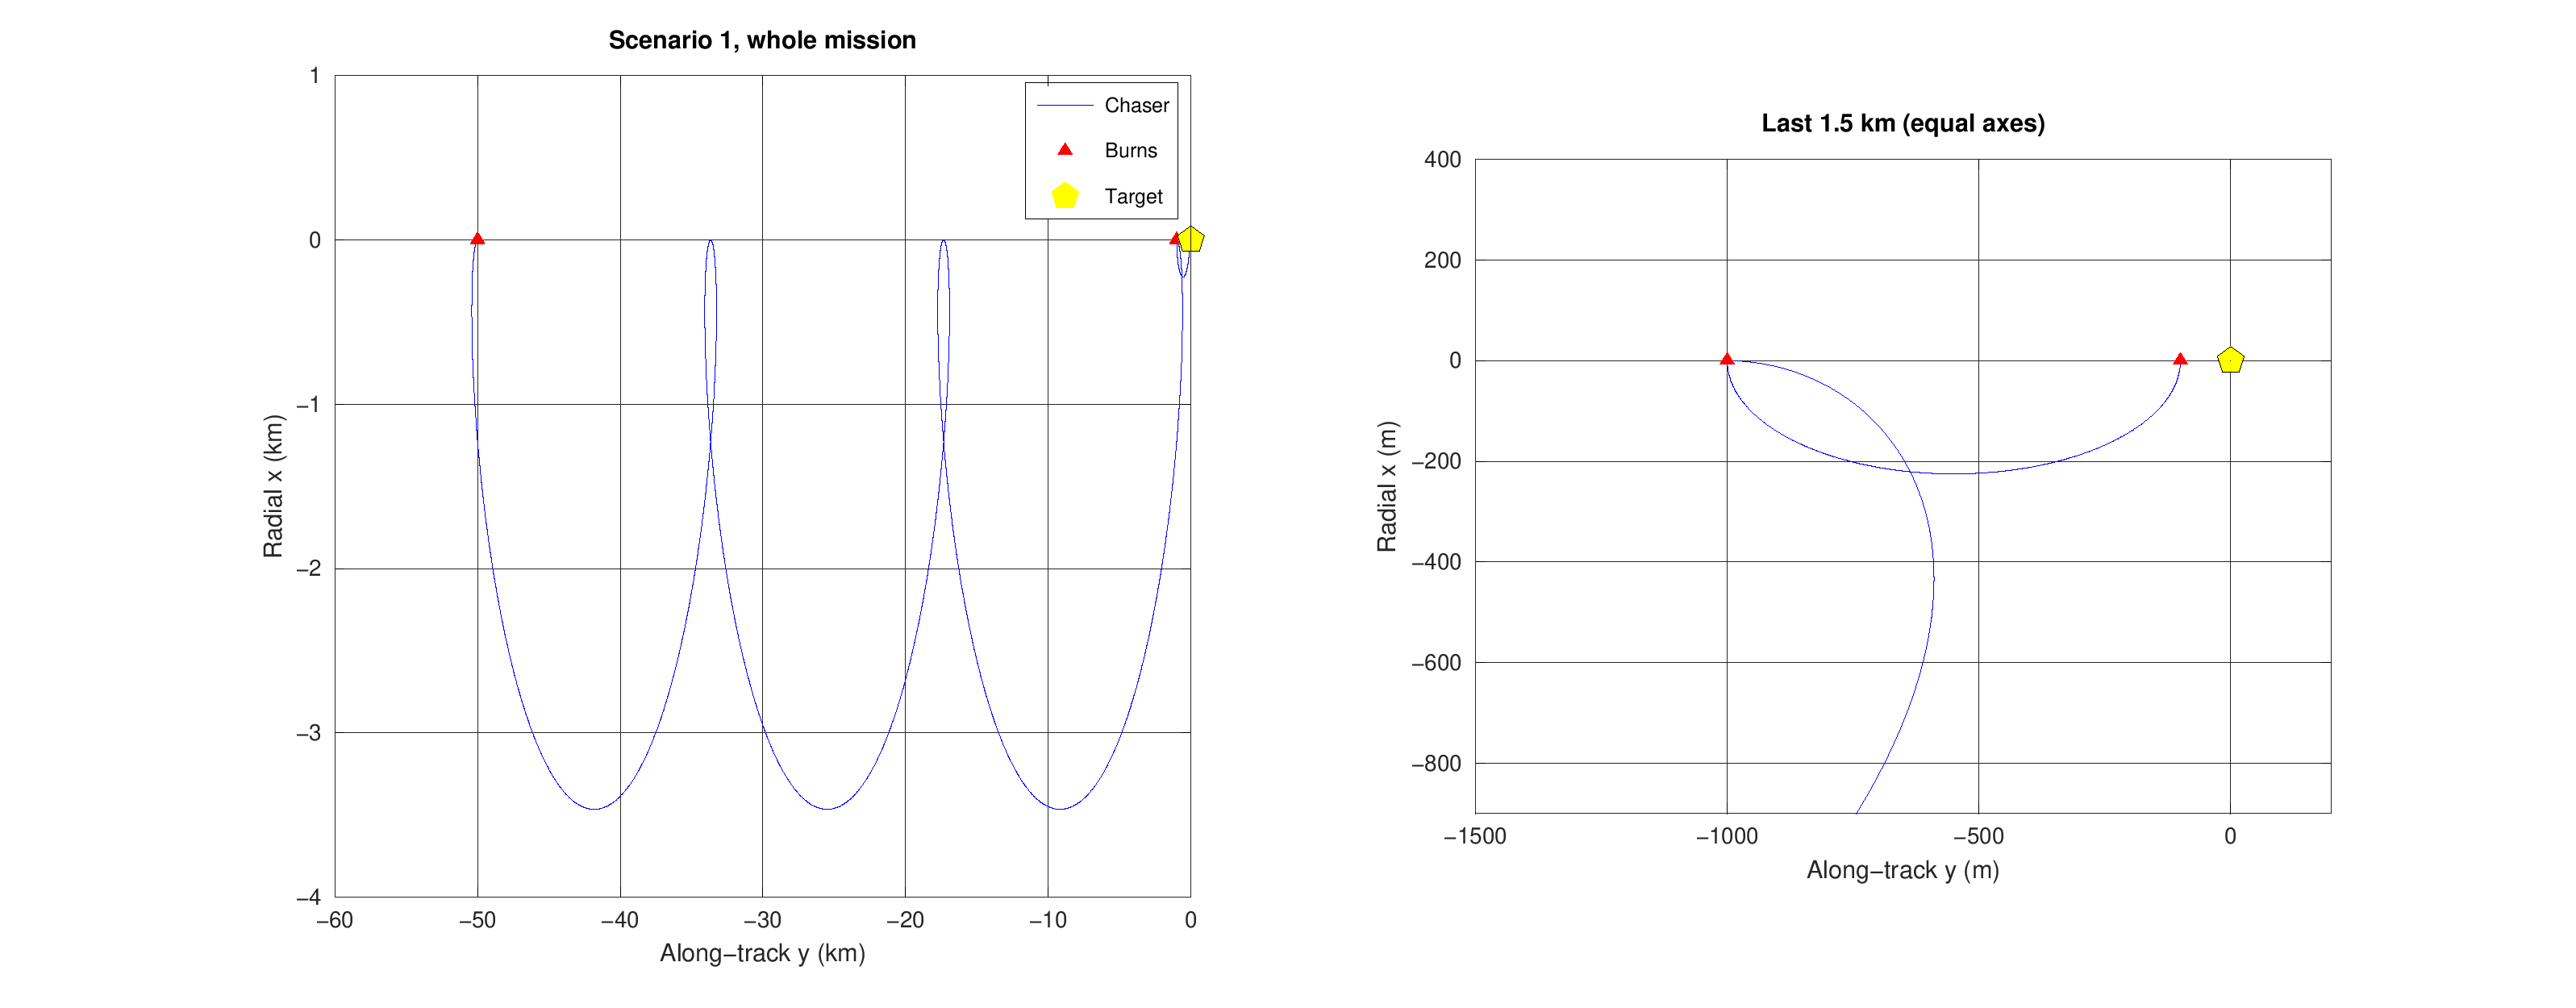
\includegraphics[width=0.95\textwidth]{s1_inplane.png}
\caption{Scenario 1 trajectory. Each phasing revolution is a loop below the
target orbit; the right panel shows the radial hop.}
\label{fig:s1}
\end{figure}

The mission costs \SI{2.770}{m/s} in \SI{5.73}{h} and uses
\SI{1.283}{kg} of propellant. The maximum relative speed is 6.858~m/s and the longest burn is 2.2~s at
$0.045\,g$, below the $0.05\,g$ limit.
The phasing cost from Eq.~(\ref{eq:trade}) is \SI{1.961}{m/s}, and the
two-impulse solver gives \SI{1.960}{m/s} (difference
\SI{0.010}{\percent}, condition number 7823).

\figref{fig:trade} shows the two-impulse cost for different transfer times.
The minima are at whole orbits, where $\Phi_{rv}$ is singular, and they
follow Eq.~(\ref{eq:trade}): 2, 3, 4, 6 and 8 revolutions cost 2.941, 1.961,
1.471, 0.980 and \SI{0.735}{m/s}. The product $\Delta V \cdot t$ is always
\SI{32.7}{km}. For example, closing the \SI{49}{km} gap with only
\SI{0.44}{m/s} would take \SI{20.6}{h}.

\begin{figure}[htbp]
\centering
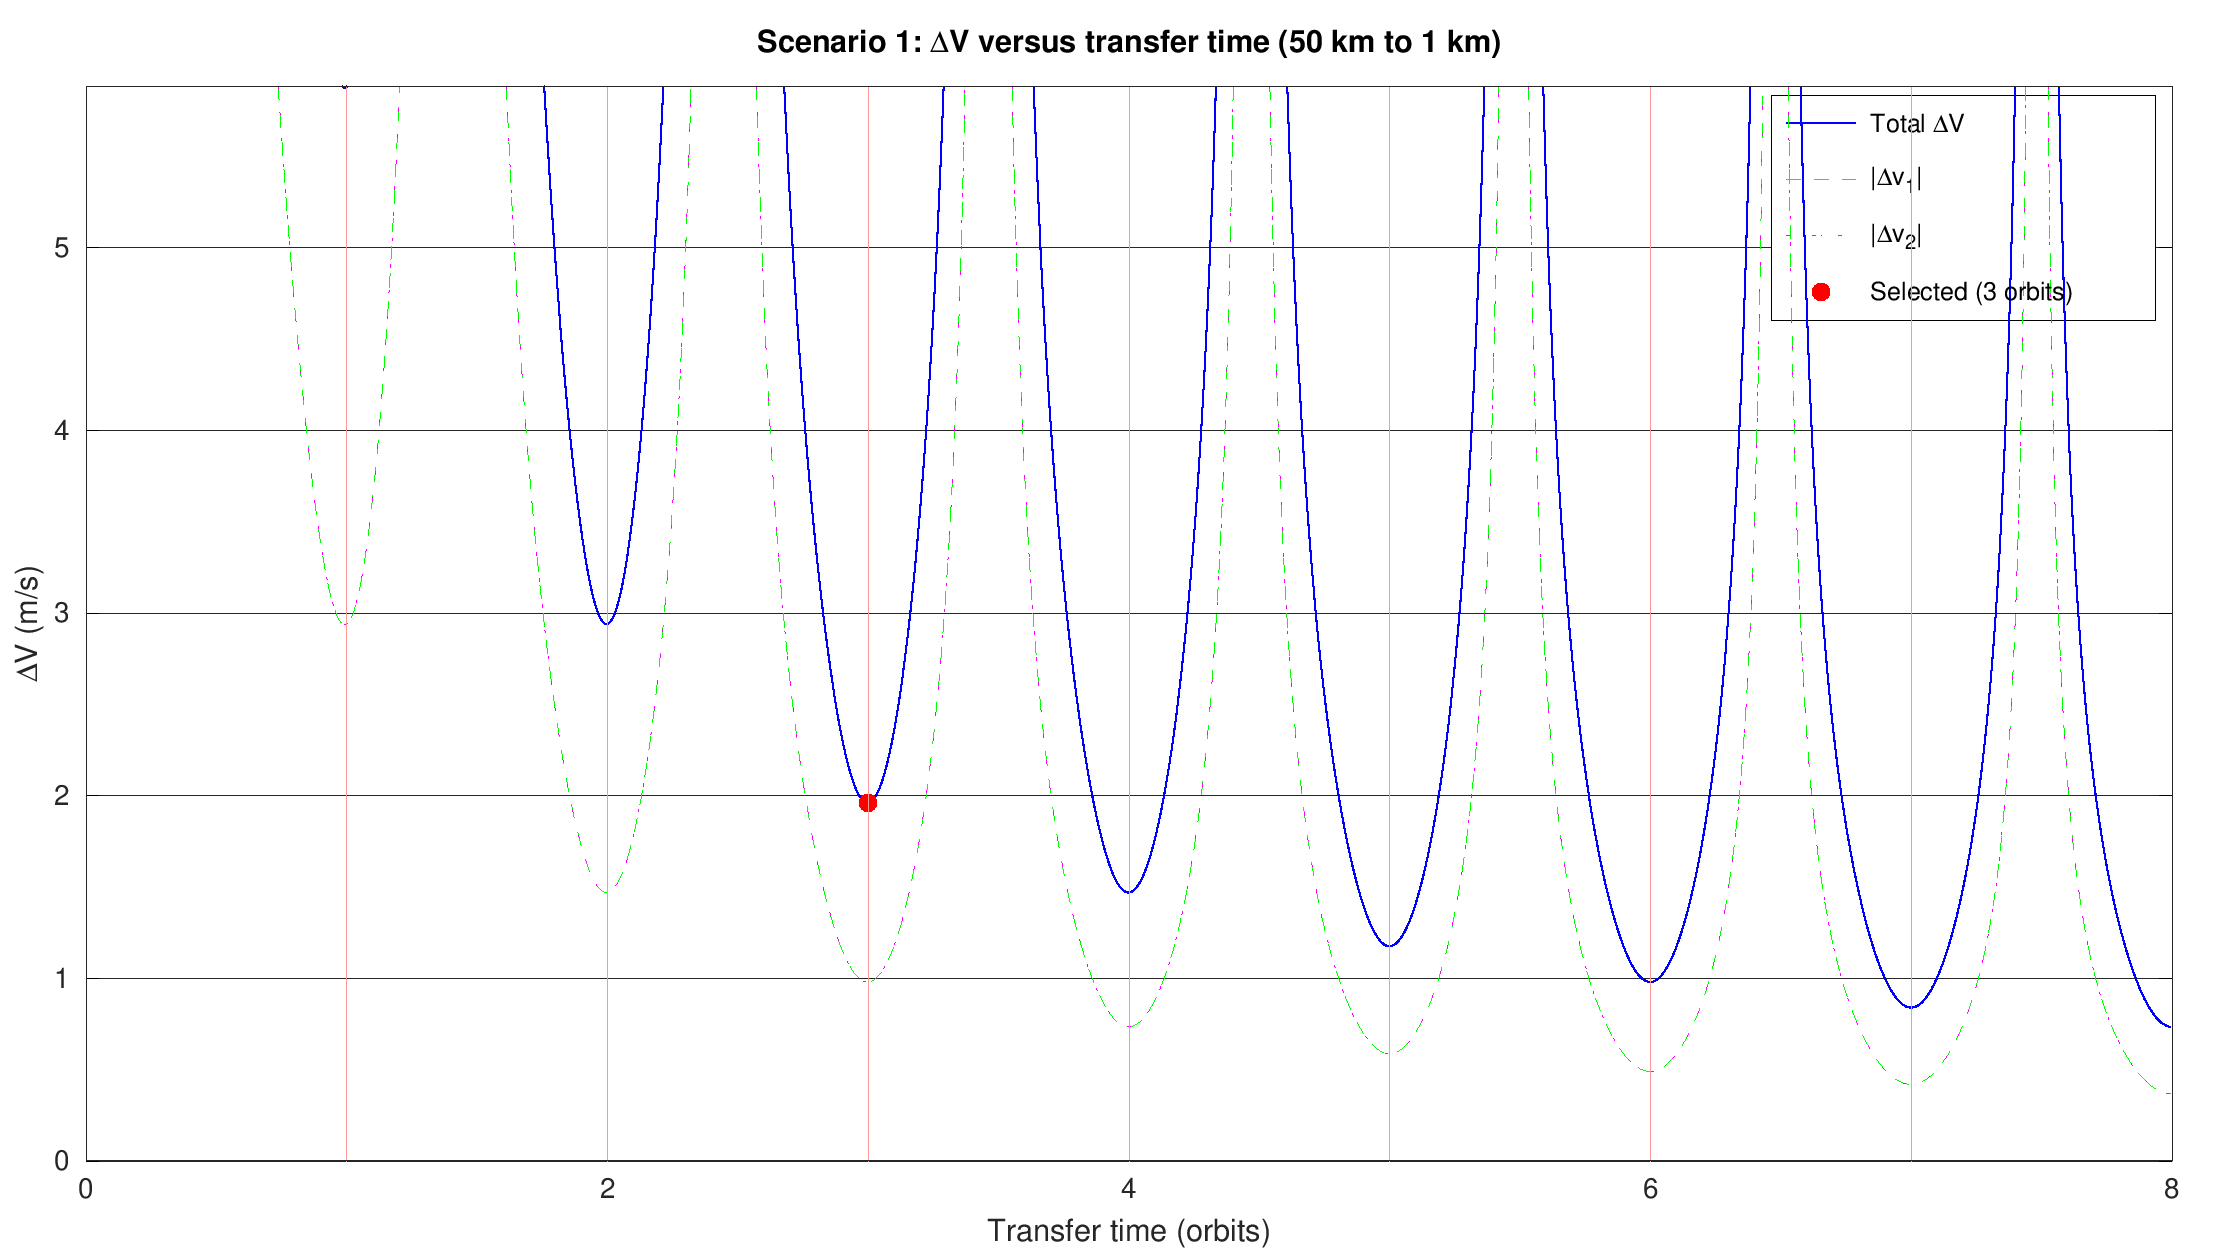
\includegraphics[width=0.85\textwidth]{s1_dv_trade.png}
\caption{Two-impulse cost versus transfer time. Vertical lines show the
singular points at whole orbits.}
\label{fig:trade}
\end{figure}

\subsection{Model Validation}

\figref{fig:valid} compares the linear prediction of the phasing coast with
the nonlinear model. In curvilinear coordinates the maximum error is
\SI{25.0}{m} (\SI{3.29}{\percent} of the distance). In Cartesian
coordinates it is \SI{21}{km}, 834 times larger. So
Cartesian HCW is fine for a few hundred meters but not for tens of
kilometers. Even the \SI{25}{m} error shows why real missions correct the
transfer during flight with new navigation data.

\begin{figure}[htbp]
\centering
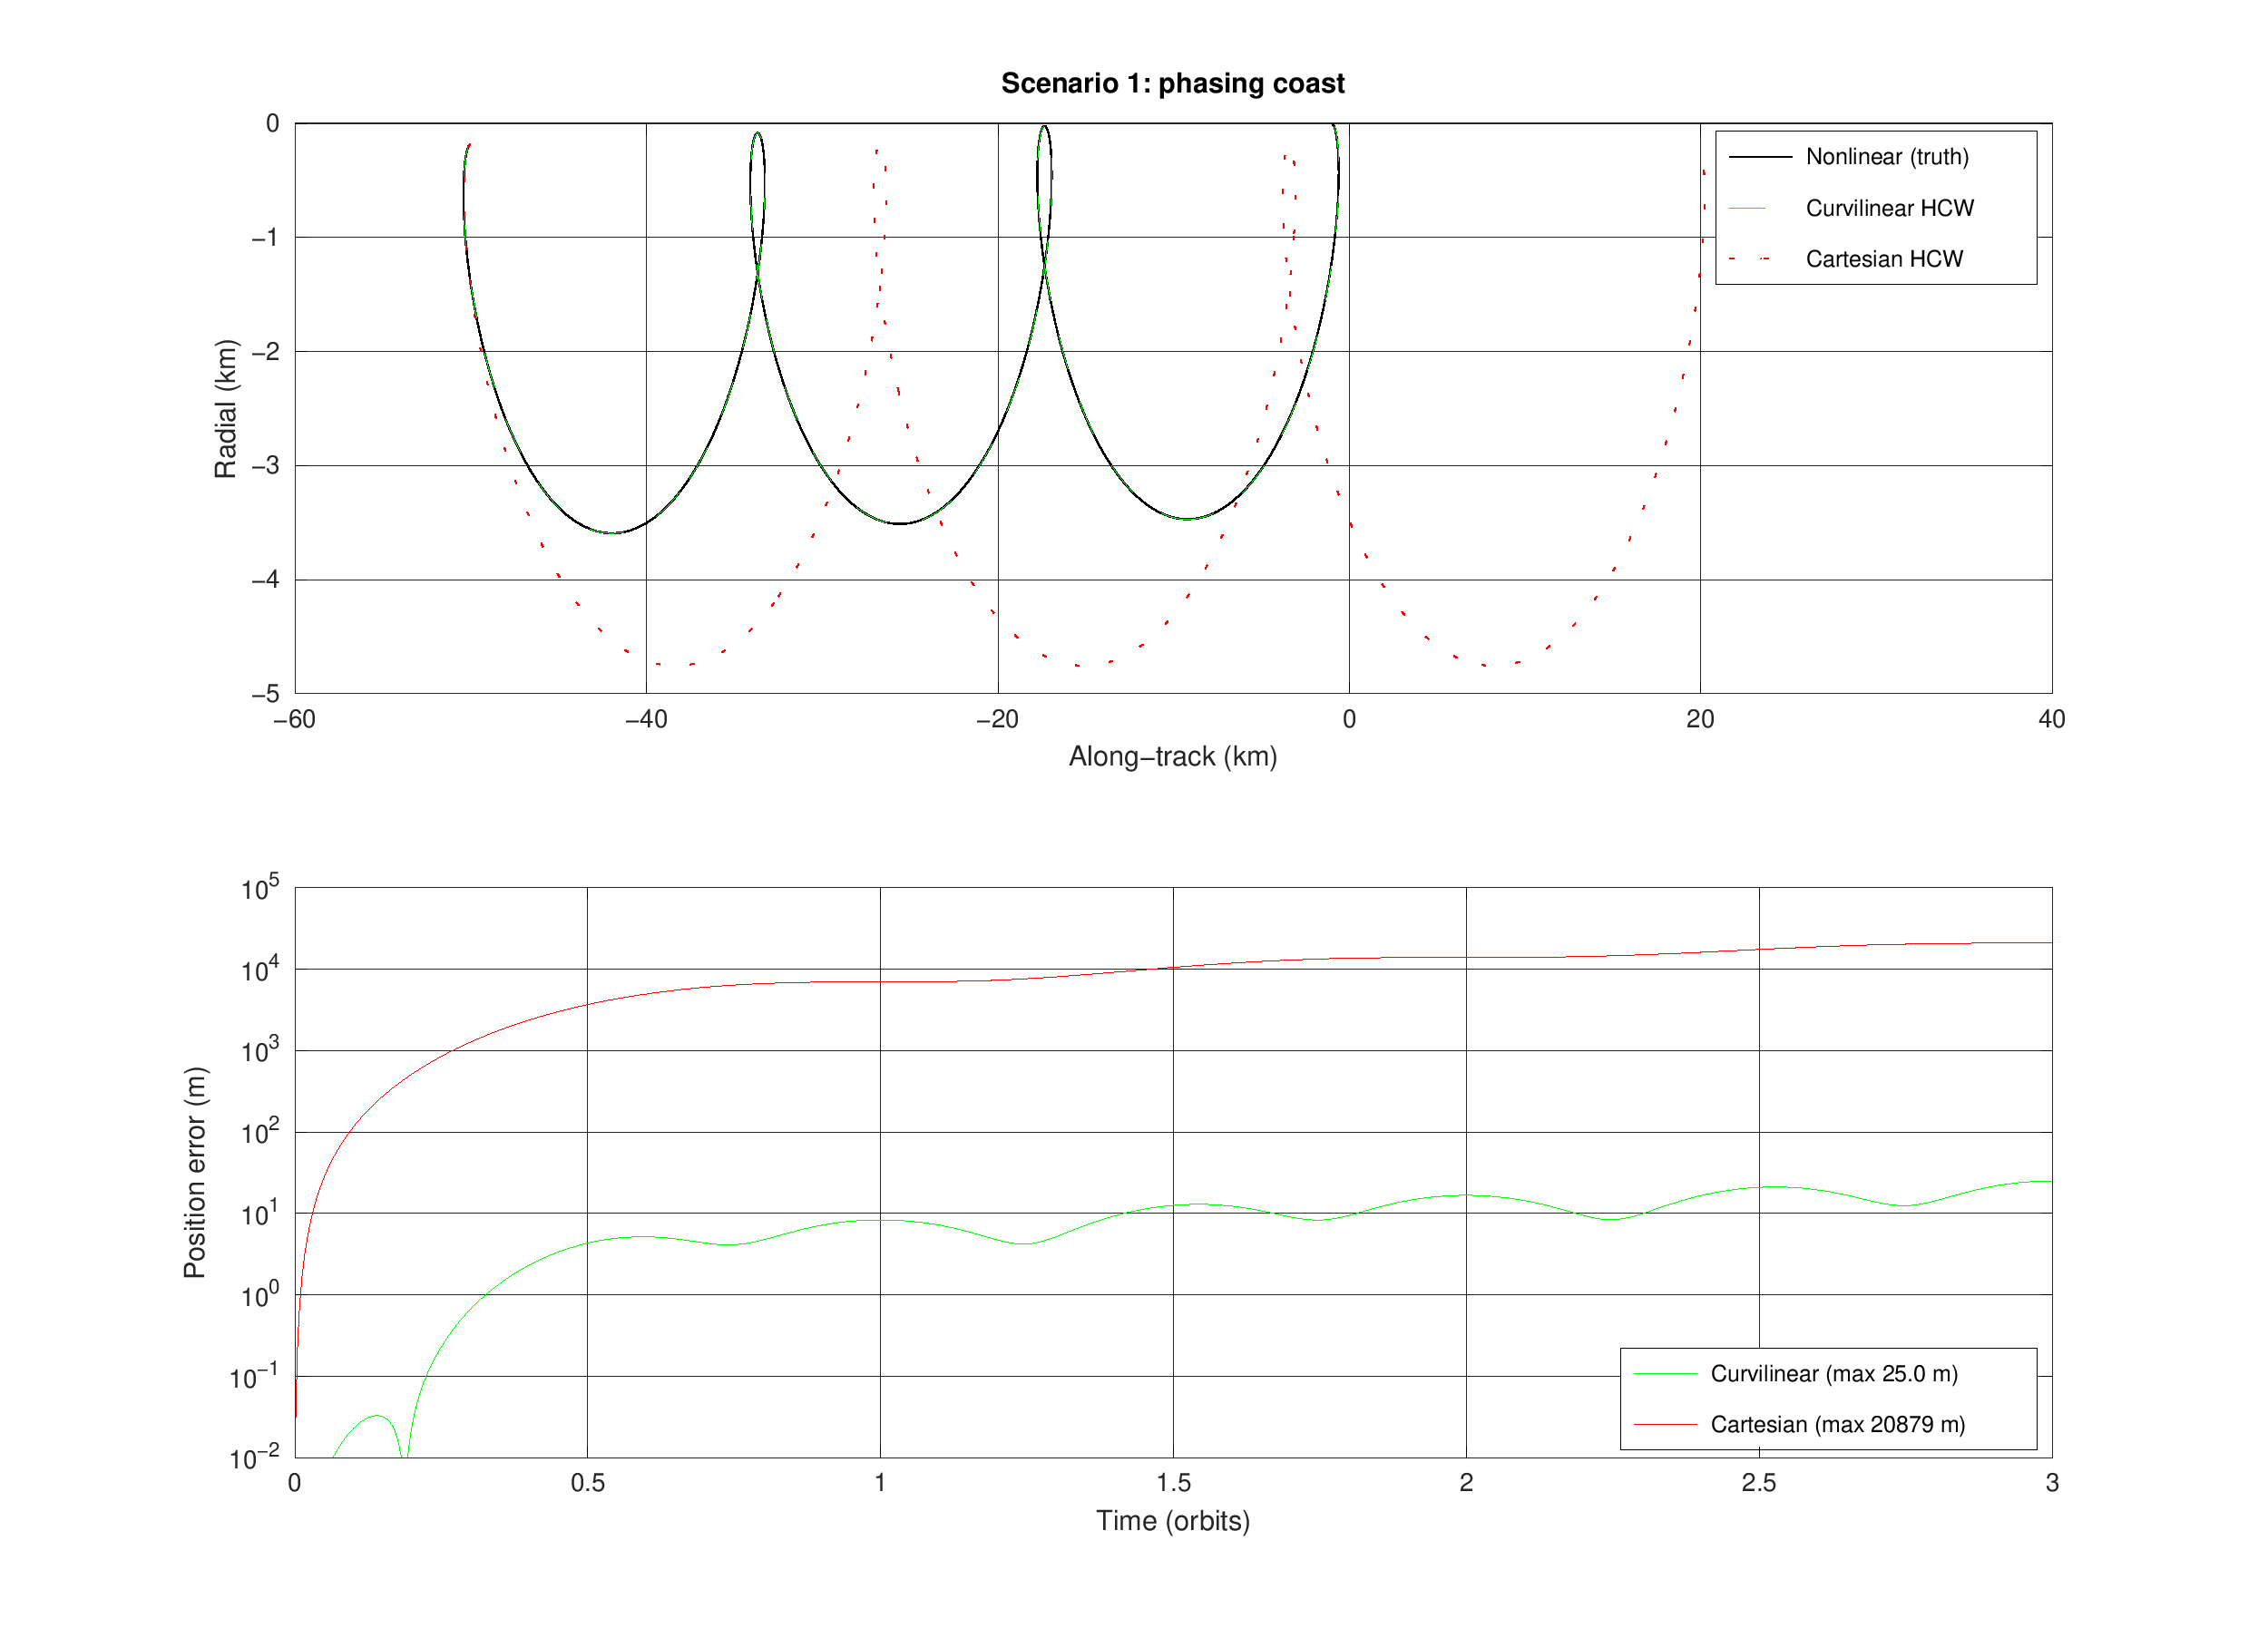
\includegraphics[width=0.95\textwidth]{s1_validation.png}
\caption{Linear HCW prediction versus the nonlinear model in curvilinear and
Cartesian coordinates (error axes are logarithmic).}
\label{fig:valid}
\end{figure}

\subsection{Scenario 2: Lower Orbit, 100 km Behind}

The chaser starts \SI{2.5}{km} below and \SI{100}{km} behind the
target with a relative inclination of \SI{0.0042}{\degree}, which gives a
\SI{500}{m} cross-track oscillation (Table~\ref{tab:s2},
\figref{fig:s2}).

\begin{table}[htbp]
\centering
\caption{Scenario 2 burns.}
\label{tab:s2}
\begin{tabular}{@{}llrrl@{}}
\toprule
Burn & Purpose & $t$ [h] & $|\Delta v|$ [m/s] & Direction \\
\midrule
-- & free drift, \SI{5.71}{h} & -- & 0 & -- \\
B1 & remove cross-track motion at the node & 0.39 & 0.566 & cross-track \\
B2 & Hohmann, first burn & 6.10 & 0.707 & prograde \\
B3 & Hohmann, second burn & 6.87 & 0.707 & prograde \\
B4, B5 & radial hop & 7.12, 7.89 & $2\times$0.2546 & radial \\
B6 & start approach & 7.97 & 0.3000 & prograde \\
\midrule
\multicolumn{3}{r}{Total} & 2.789 & \\
\bottomrule
\end{tabular}
\end{table}

\begin{figure}[htbp]
\centering
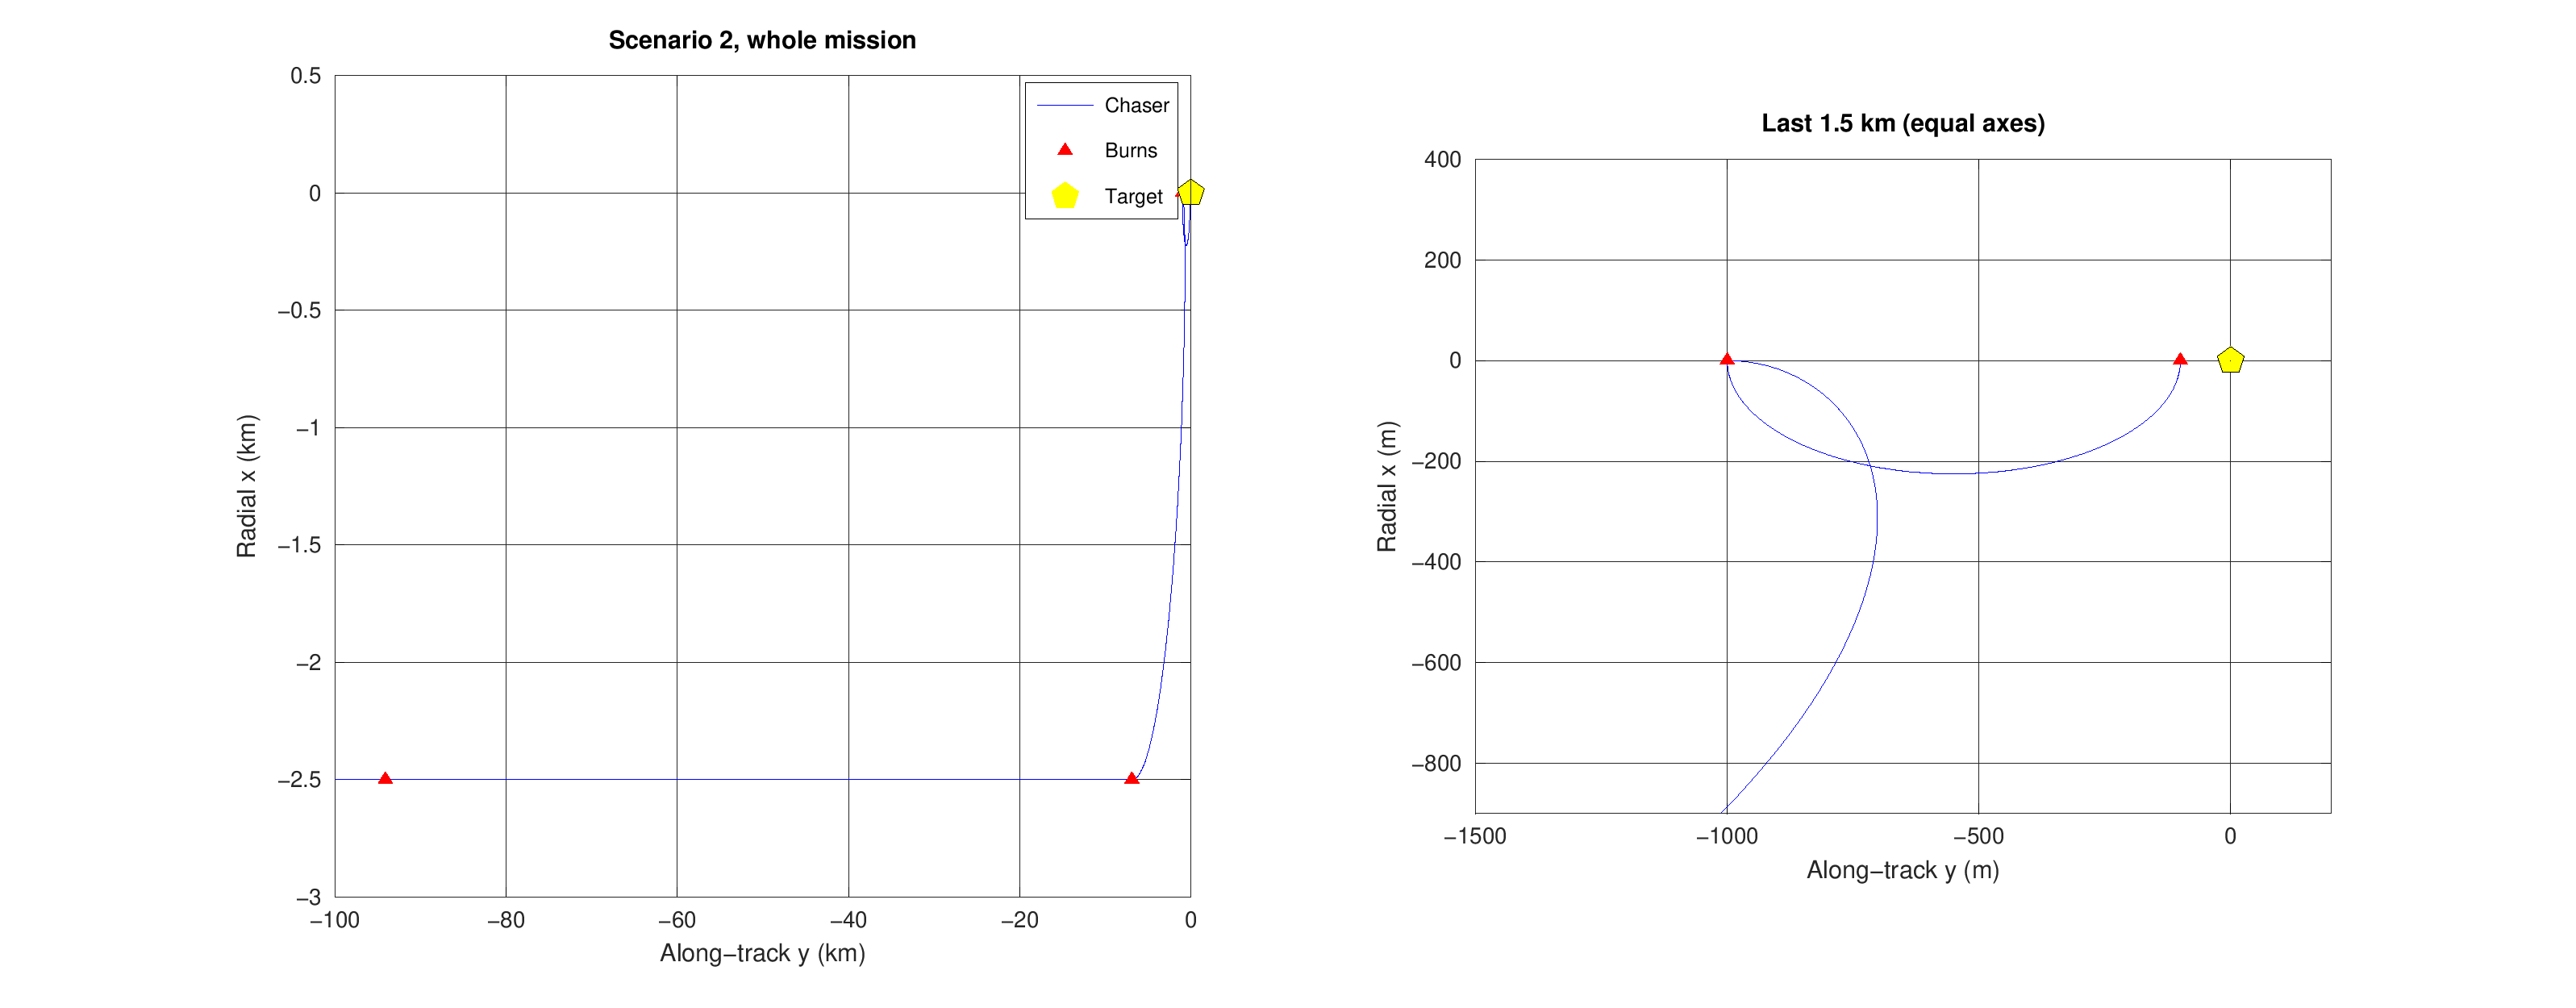
\includegraphics[width=0.95\textwidth]{s2_inplane.png}
\caption{Scenario 2 trajectory. The long line is the free drift below the
target orbit; the right panel shows the Hohmann transfer and radial hop.}
\label{fig:s2}
\end{figure}

In \SI{5.71}{h} of free drift the chaser closes \SI{93}{km}, which is
\SI{93}{\percent} of the distance, without propellant. Closing the same gap
by phasing in the same time would cost \SI{3.2}{m/s}. The cross-track motion
is removed with one burn of \SI{0.566}{m/s} at the node, where $z = 0$.
Out-of-plane motion is expensive: this burn removes only \SI{500}{m} of
offset, while \SI{0.509}{m/s} in the radial hop moves the chaser
\SI{900}{m}.

I stopped the drift at \SI{6.89}{km}, where a purely tangential Hohmann
transfer ends at the waypoint. It costs \SI{1.414}{m/s}, equal to the
formula value. When I first stopped the drift at \SI{5}{km}, the transfer
needed a radial part and cost \SI{25}{\percent} more. During the drift the
curvilinear model has an error of \SI{167.5}{m}; correcting the transfer
from the true state costs only \SI{0.0107}{m/s}. Scenario~2 costs
\SI{2.789}{m/s} in \SI{7.97}{h} and uses \SI{1.292}{kg} of propellant.

\subsection{Scenario 3: Terminal Approach}

The controller starts at \SI{100}{m} on the V-bar with an initial
error of \SI{1.5}{m} radial, \SI{1.0}{m} cross-track and a few mm/s in
velocity (\figref{fig:s3}, Table~\ref{tab:contact}).

\begin{figure}[htbp]
\centering
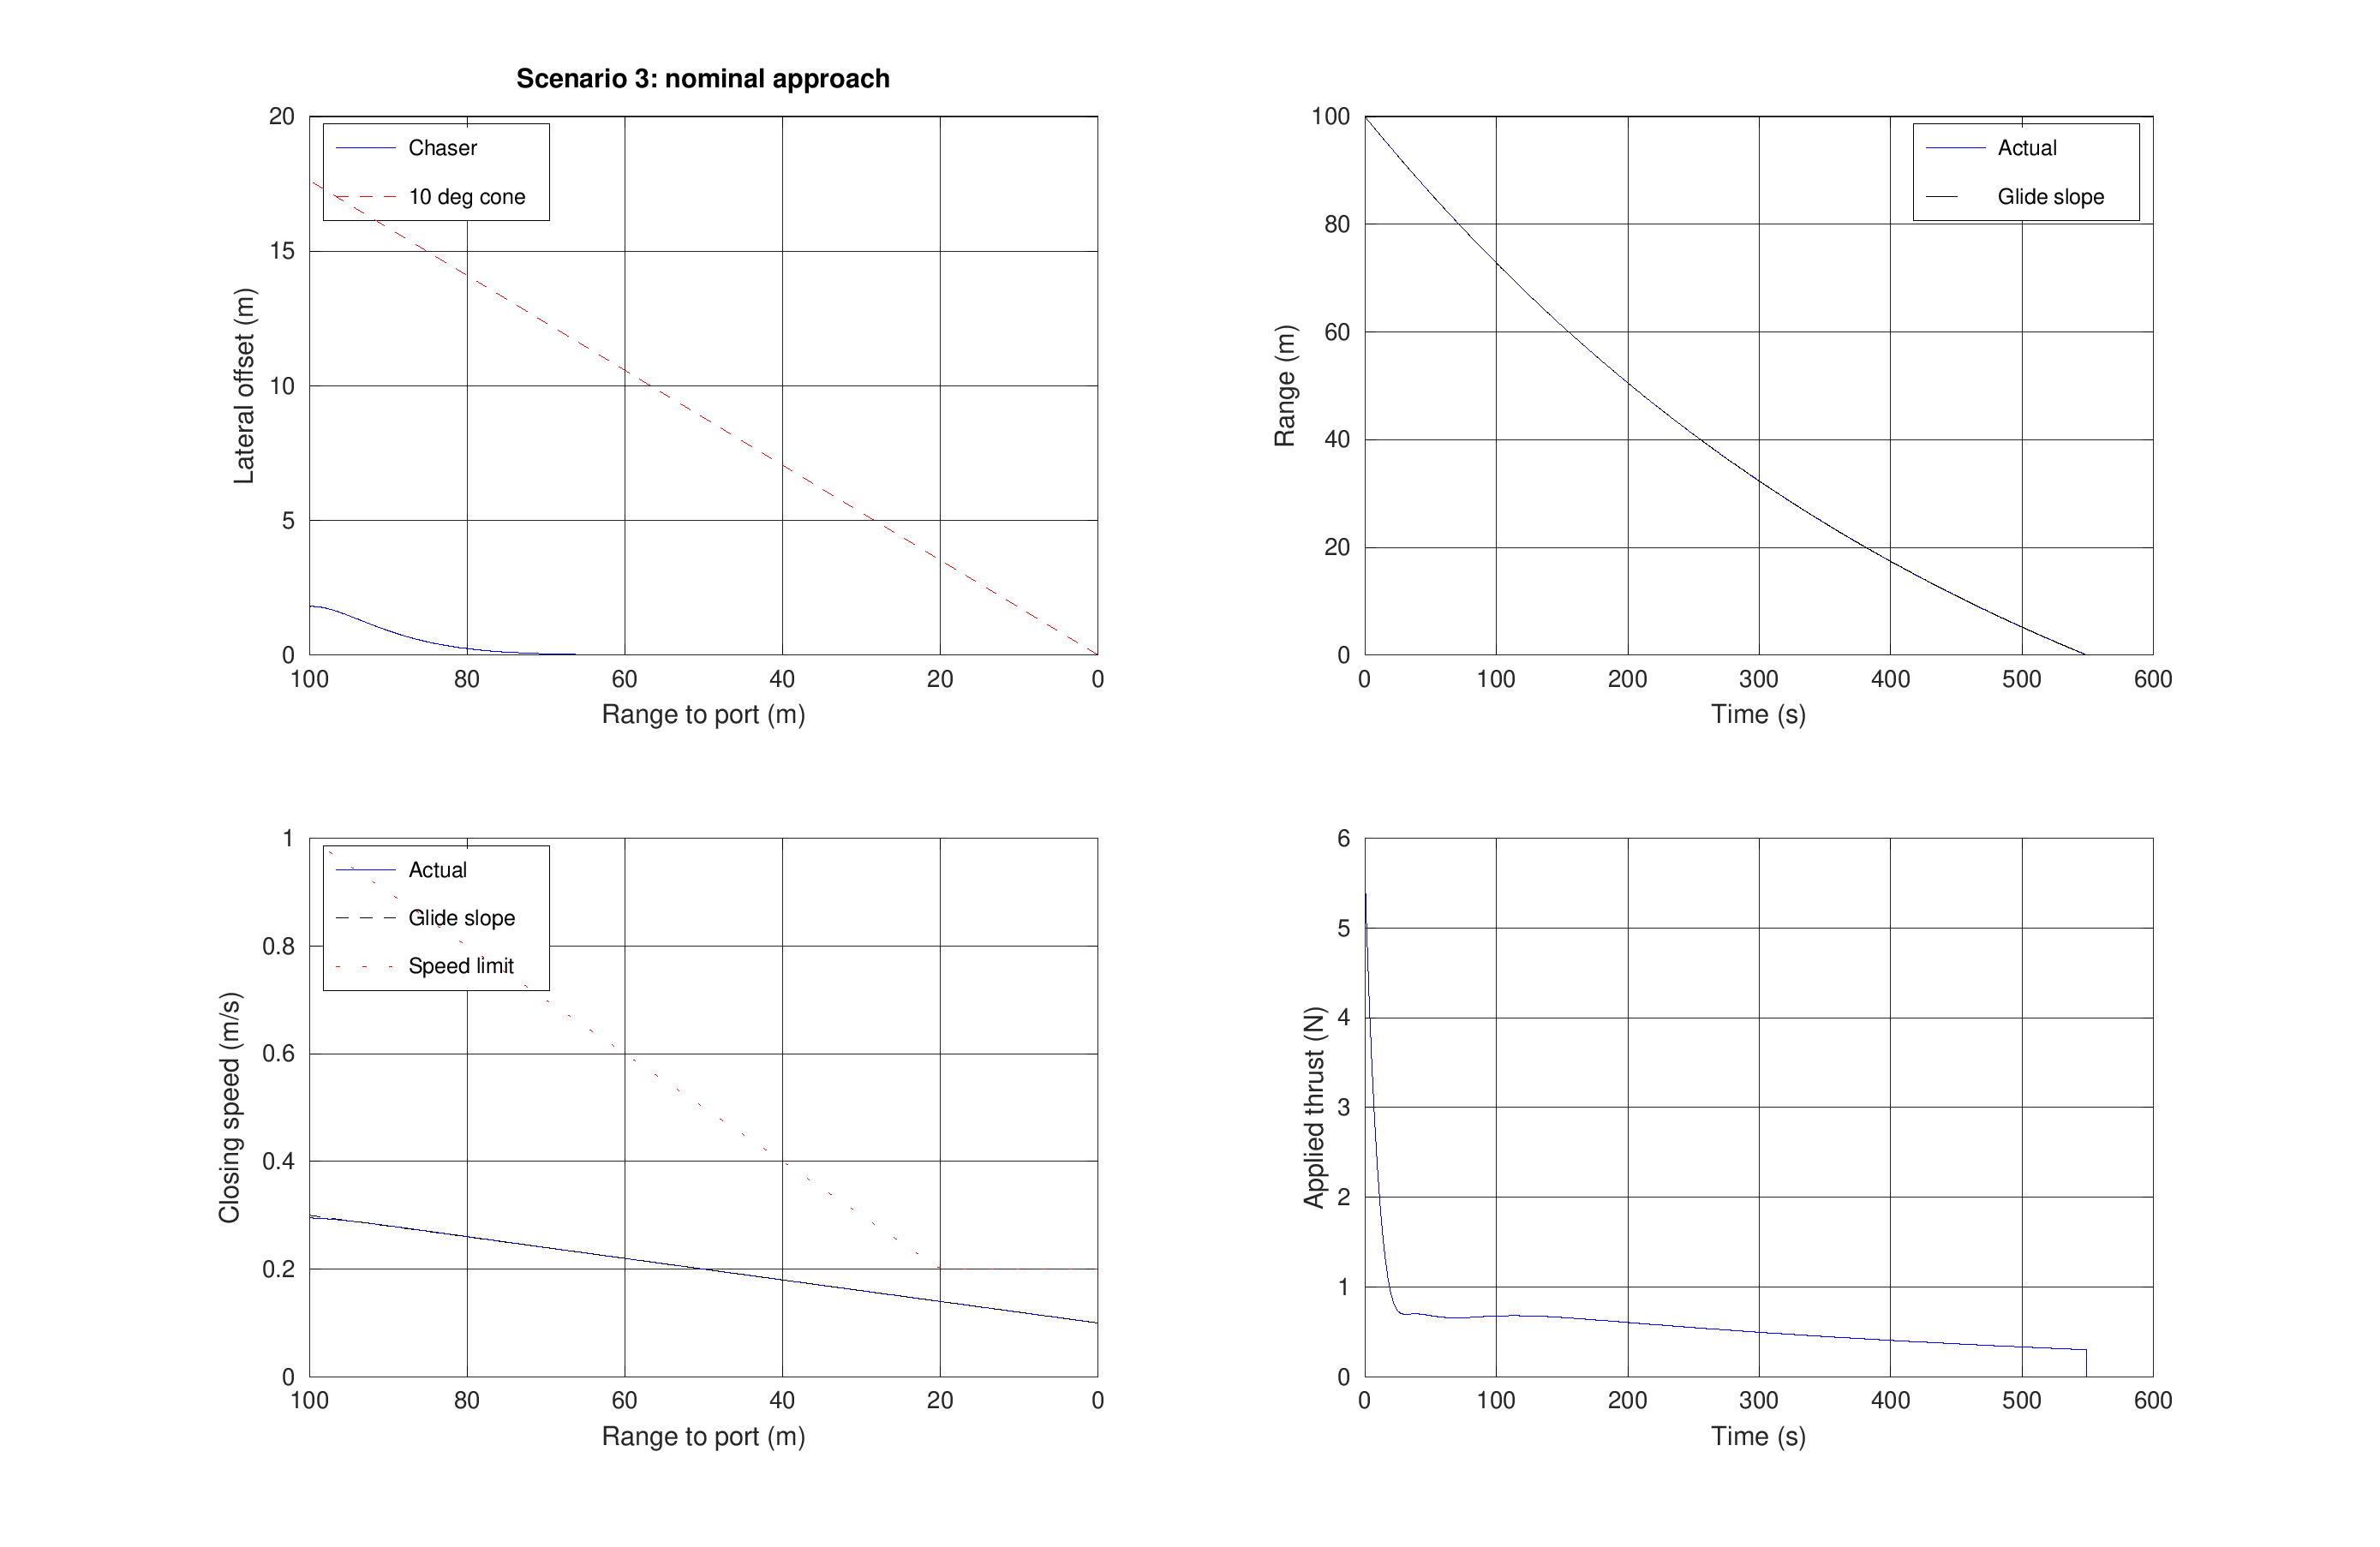
\includegraphics[width=0.95\textwidth]{s3_dashboard.png}
\caption{Scenario 3, nominal approach. The chaser stays inside the cone and
below the speed limit and reaches the port at \SI{0.100}{m/s}.}
\label{fig:s3}
\end{figure}

\begin{table}[htbp]
\centering
\caption{Contact conditions and typical soft-docking limits.}
\label{tab:contact}
\begin{tabular}{@{}lrr@{}}
\toprule
Quantity & Result & Limit \\
\midrule
Axial contact speed & \SI{0.100}{m/s} & \SIrange{0.05}{0.15}{m/s} \\
Lateral contact speed & \SI{0.0000}{m/s} & $< \SI{0.05}{m/s}$ \\
Lateral miss & \SI{0.000}{m} & $< \SI{0.10}{m}$ \\
Maximum cone angle & \SI{1.04}{\degree} & $< \SI{10}{\degree}$ \\
\bottomrule
\end{tabular}
\end{table}

Contact happens after \SI{549}{s}, within \SI{0.02}{\percent} of
Eq.~(\ref{eq:glide}). The lateral speed and miss are zero because in this
case there is no noise and the feedforward cancels the orbital coupling
exactly, so the initial error decays long before contact. The approach costs
\SI{0.325}{m/s}, and the peak thrust is \SI{5.66}{N}, below the
\SI{20}{N} limit.

\paragraph{Gain study.} Table~\ref{tab:gains} and \figref{fig:gains} compare
four gain sets. The last one is a much faster design that I included for
comparison.

\begin{table}[htbp]
\centering
\caption{Gain study (thrust is the commanded value before saturation).}
\label{tab:gains}
\begin{tabular}{@{}rrrrrr@{}}
\toprule
$K_p$ [s$^{-2}$] & $K_d$ [s$^{-1}$] & $\omega_n$ & $\zeta$ & $v_c$ [m/s] & peak thrust [N] \\
\midrule
$2.5\times10^{-4}$ & 0.032 & 0.016 & 1.00 & 0.100 & 1.3 \\
$\bm{2.5\times10^{-3}}$ & \textbf{0.100} & \textbf{0.050} & \textbf{1.00} & \textbf{0.100} & \textbf{5.7} \\
$2.5\times10^{-3}$ & 0.040 & 0.050 & 0.40 & 0.100 & 5.3 \\
$1.0\times10^{-1}$ & 0.500 & 0.316 & 0.79 & 0.100 & 183.8 \\
\bottomrule
\end{tabular}
\end{table}

\begin{figure}[htbp]
\centering
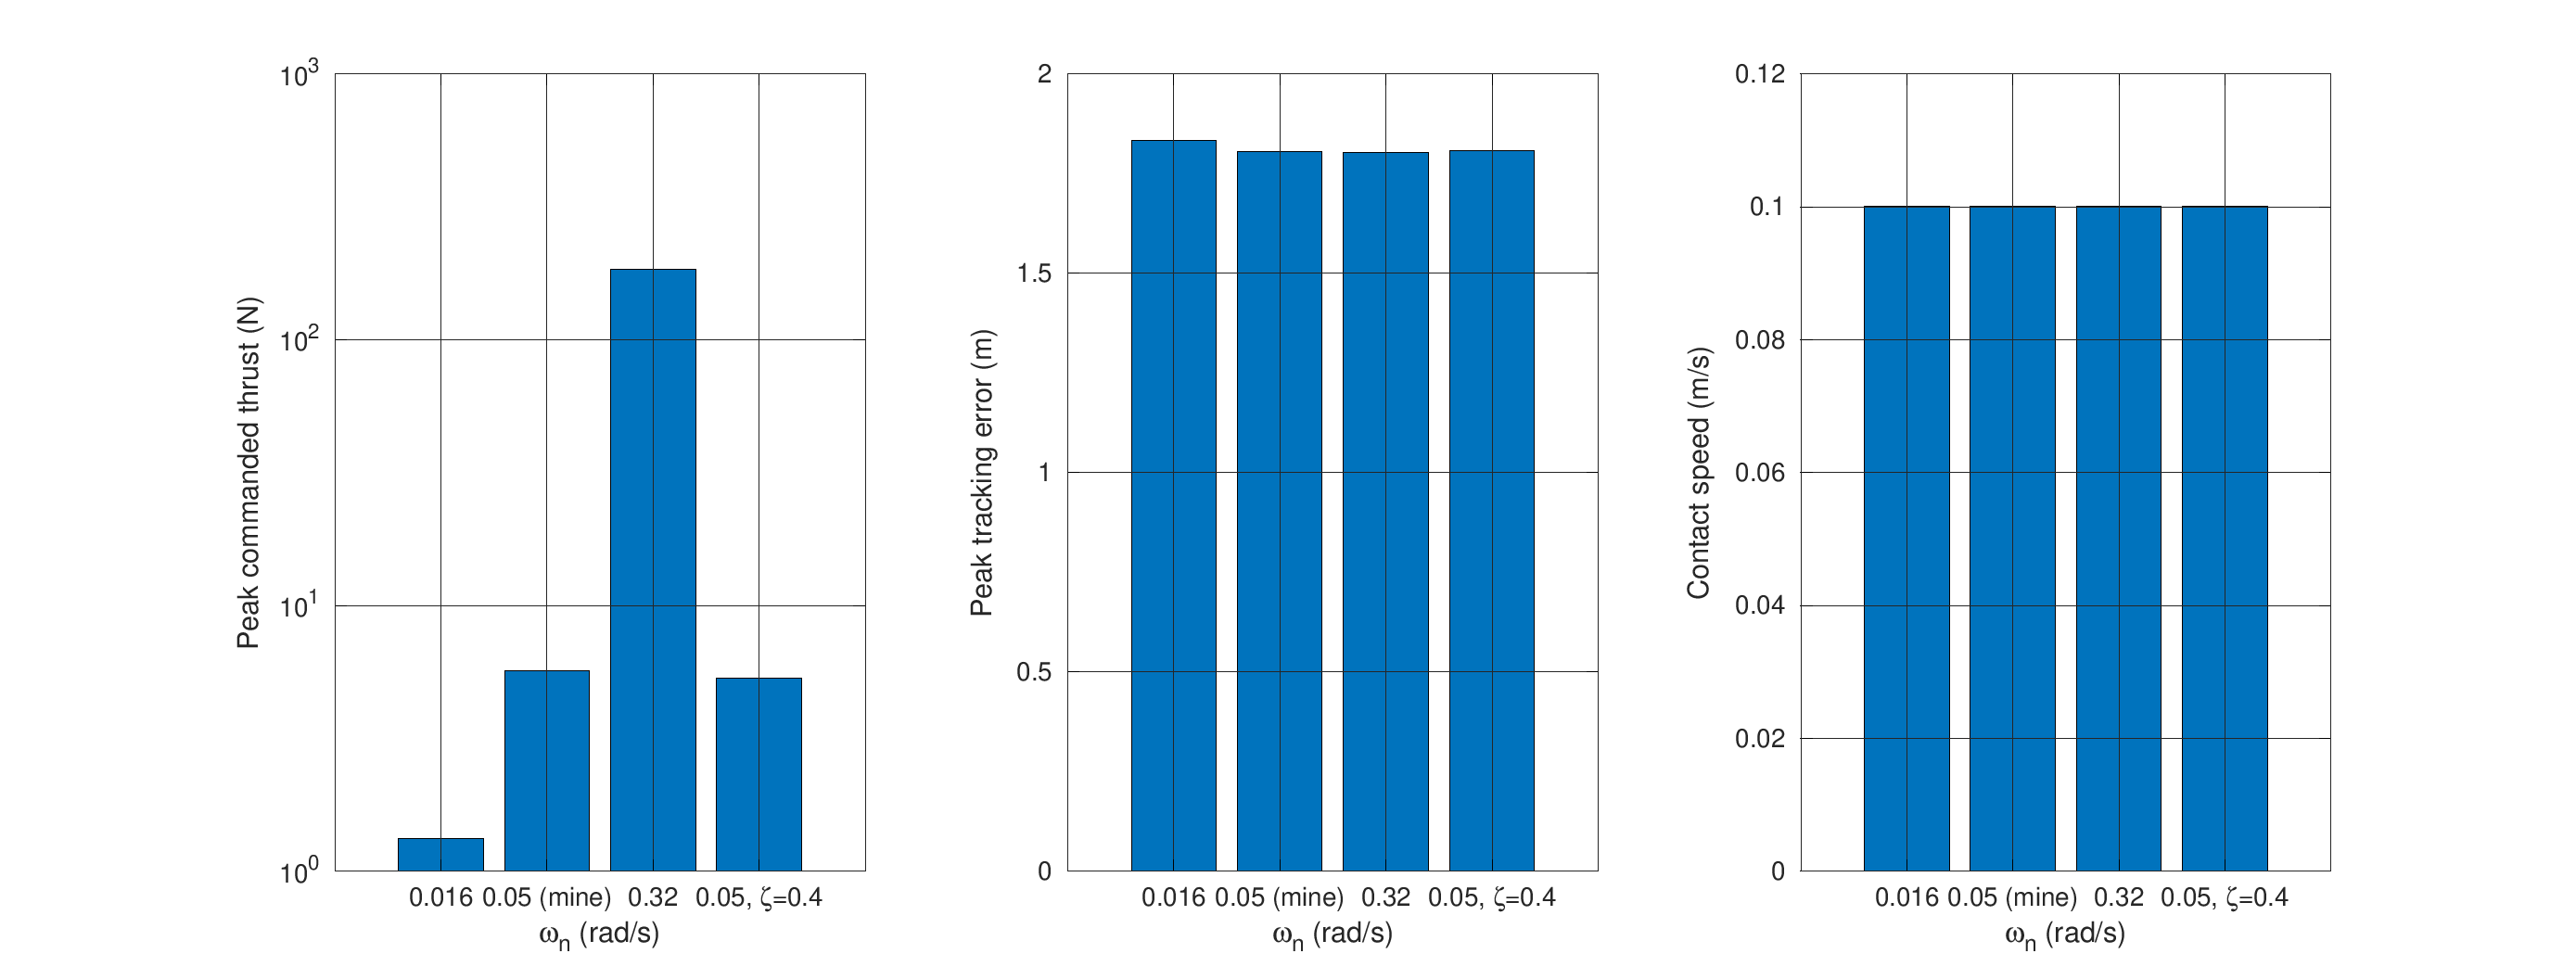
\includegraphics[width=0.9\textwidth]{s3_gain_trade.png}
\caption{Gain study. The peak thrust changes by two orders of magnitude, the
contact accuracy almost not.}
\label{fig:gains}
\end{figure}

The gains $K_p = 0.1$, $K_d = 0.5$ give a time constant of about \SI{3}{s}
for a nine-minute maneuver. This design asks for \SI{183.8}{N},
32 times more than mine, but the contact speed and miss are the
same. A faster controller does not help, because the reference is smooth and
there is no fast disturbance. The slowest design needs only \SI{1.3}{N}, but
its \SI{63}{s} time constant leaves less margin for larger errors. My choice
has a \SI{20}{s} time constant, between the \SI{550}{s} approach and the
\SI{10}{Hz} controller.

\paragraph{Navigation noise.} With \SI{2}{cm} position noise and
\SI{5}{mm/s} velocity noise ($1\sigma$), the contact is still good:
\SI{0.0993}{m/s} axial speed and \SI{0.0069}{m} lateral miss. But the
delta-V grows from \SI{0.325}{} to \SI{0.554}{m/s}, about
\SI{70}{\percent} more, because the derivative term turns velocity noise into
many small firings. Real flight software filters the measurements first.

\paragraph{Failure case.} To test the safety monitor, I reduced the thrust to
\SI{0.4}{N} and added a \SI{55}{mm/s} cross-track speed at the start
(\figref{fig:abort}). The controller asks for \SI{37.0}{N} and stays
saturated, the lateral offset grows while the cone narrows, and after
\SI{131}{s} the chaser leaves the cone \SI{11.0}{m} off axis.
The monitor stops the approach, which is the correct decision.

\begin{figure}[htbp]
\centering
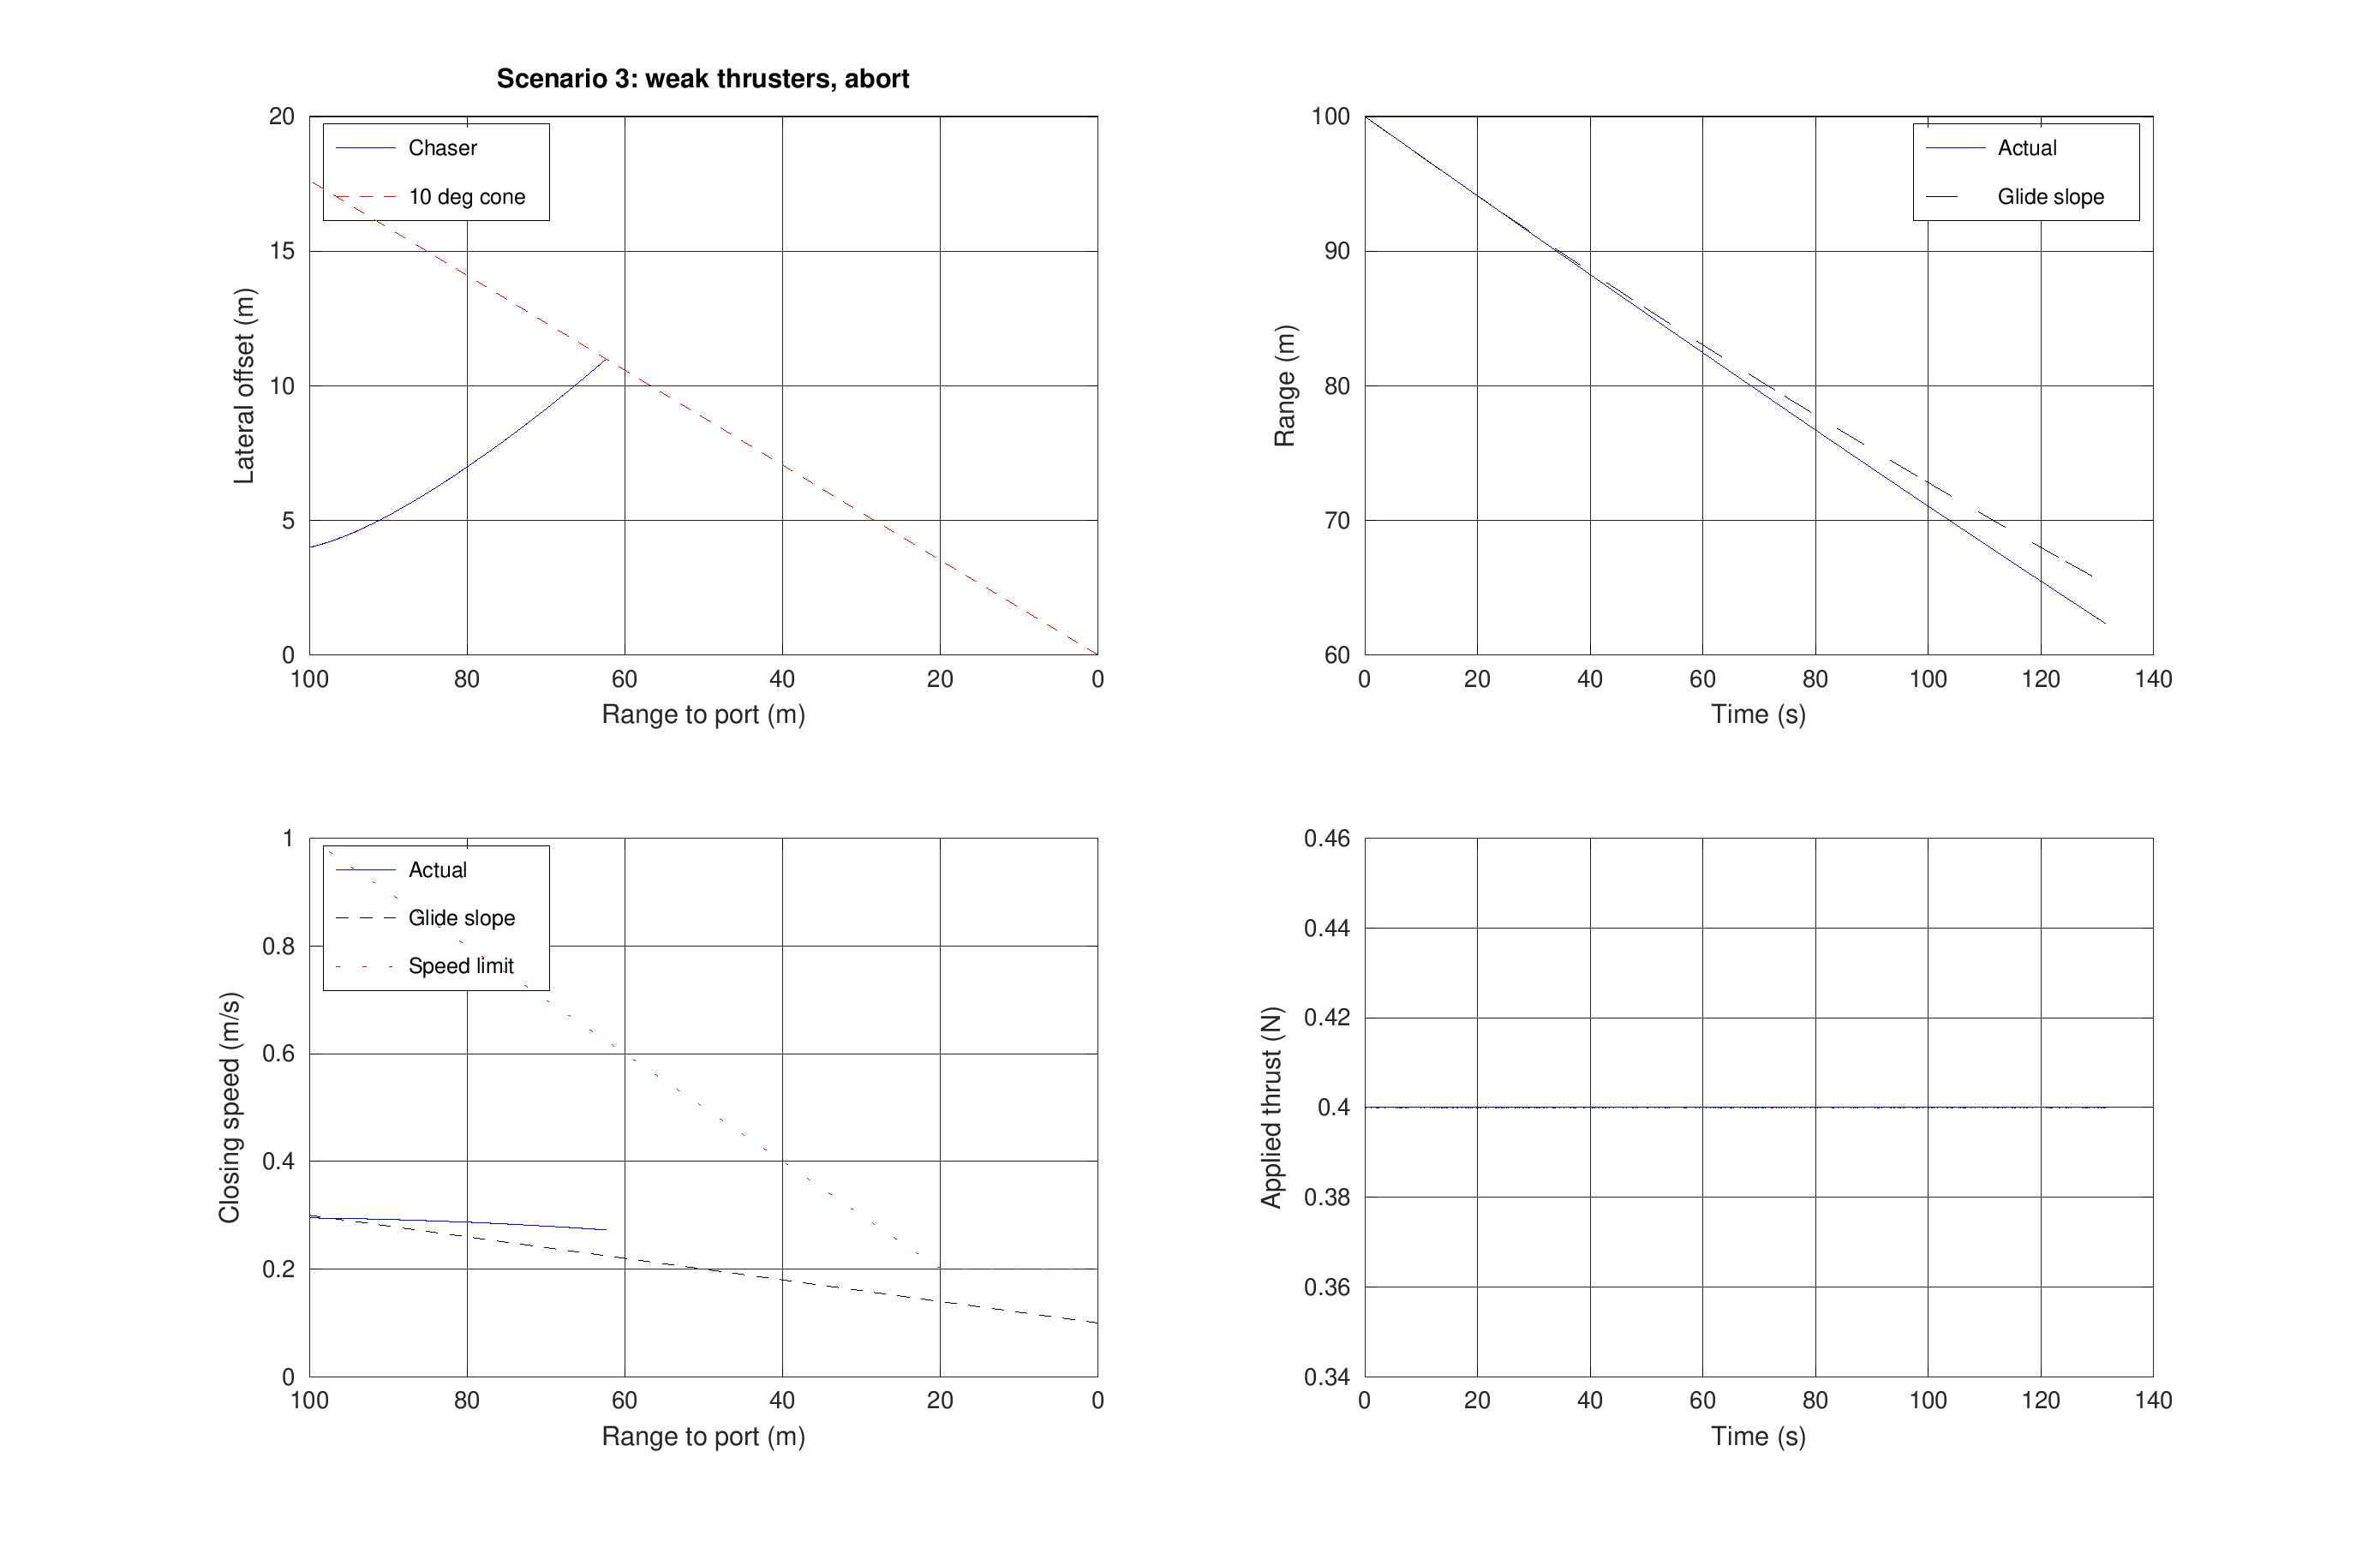
\includegraphics[width=0.95\textwidth]{s3_dashboard_abort.png}
\caption{Scenario 3, failure case with \SI{0.4}{N} thrusters. The chaser
leaves the cone after \SI{131}{s} and the approach is aborted.}
\label{fig:abort}
\end{figure}

\subsection{Full Mission}

Scenario~2 plus Scenario~3 needs \SI{3.114}{m/s} in \SI{8.12}{h} and
\SI{1.442}{kg} of propellant, \SI{0.14}{\percent} of the vehicle mass. The
propellant is small because the mission takes eight hours. From
Eq.~(\ref{eq:trade}), doing the same profile in two hours would make the
phasing about four times more expensive.

% =====================================================================
\section{Conclusions}

\begin{enumerate}[leftmargin=2.2em,itemsep=0pt]
  \item A full guidance chain from \SI{100}{km} to contact was built and
        tested. The chaser docks at \SI{0.100}{m/s} for \SI{3.114}{m/s} in
        \SI{8.12}{h}.
  \item The far-range cost follows $\Delta V\cdot t = \tfrac23\Delta y$, and the
        cheapest transfers are at the singular points of the targeting matrix.
  \item Cartesian HCW coordinates do not work beyond a few kilometers: at
        \SI{50}{km} the error after three orbits is \SI{21}{km},
        compared with \SI{25.0}{m} in curvilinear coordinates.
  \item Starting below the target closes \SI{93}{\percent} of the distance for
        free.
  \item A much faster controller needs 32 times more thrust and
        does not improve the contact accuracy.
  \item Navigation noise increases the terminal propellant by
        \SI{70}{\percent}. The safety monitor correctly aborts the failure case.
\end{enumerate}

\textit{Limitations.} The target orbit is circular, the chaser is a point
mass with perfect attitude, far-range burns are impulsive, and the nonlinear
model has no $J_2$ or drag. Next steps would be elliptic target orbits,
$J_2$ and drag, finite burns, coupling with the attitude controller of my
CubeSat project, and Monte Carlo runs.

% =====================================================================
\begin{thebibliography}{9}
\setlength{\itemsep}{0pt}
\small

\bibitem{fehse}
Fehse, W., \textit{Automated Rendezvous and Docking of Spacecraft},
Cambridge University Press, Cambridge, 2003.

\bibitem{clohessy}
Clohessy, W.~H., and Wiltshire, R.~S., ``Terminal Guidance System for
Satellite Rendezvous,'' \textit{Journal of the Aerospace Sciences}, Vol.~27,
No.~9, 1960, pp.~653--658.

\bibitem{curtis}
Curtis, H.~D., \textit{Orbital Mechanics for Engineering Students}, 4th ed.,
Butterworth-Heinemann, Oxford, 2020.

\bibitem{vallado}
Vallado, D.~A., \textit{Fundamentals of Astrodynamics and Applications},
4th ed., Microcosm Press, Hawthorne, CA, 2013.

\bibitem{alfriend}
Alfriend, K.~T., Vadali, S.~R., Gurfil, P., How, J.~P., and Breger, L.~S.,
\textit{Spacecraft Formation Flying: Dynamics, Control and Navigation},
Elsevier, Oxford, 2010.

\end{thebibliography}

\end{document}
